\chapter{Experimental methods}
\section{Introduction}
This chapter provides an overview of the materials, techniques, and methods used in the experimental work performed in this thesis and outlines the procedures used in the following chapters. 

\section{Preparation of gas standards} \label{gasprep}
Gas standards of hydrogen were prepared gravimetrically in 10 litre cylinders (BOC, UK) in accordance with \cite{InternationalStandardISO6142-1:2015} from pure hydrogen (Air Products, UK), nitrogen (Air Products), carbon monoxide (Scott Speciality Gases, UK), methane (CK Gases, UK) and krypton (BOC, UK). Any impurities that were detected in these pure gases were quantified and these values were then incorporated into the final determination of the gas mixture compositions and uncertainties. 

The 10 liter cylinder was evacuated to $1 \times 10^{-6} mBar$ using a scroll pump followed by a turbo pump. This pressure ensureds that any residual gas within the cylinder will not contribute towards the uncertainty of the final mixture. \cite{InternationalStandardISO6142-1:2015} The target masses of each impurity desired in the gas mixture was then calculated using equation \ref{targetmass}where $M_\Omega$ is calculated using equation \ref{targetmass1}

\begin{equation}\label{targetmass} 
  m_j = \frac{y_k \times M_k}{\sum_{i=1}^{q}y_i \times M_i}\times m_\Omega
\end{equation}

\begin{equation}\label{targetmass1}
  m_\Omega = \frac{p_{F, \Omega} \times V_{cyl}}{Z_\Omega \times R \times T_F}\sum_{i=1}^{q}y_i \times M_i
\end{equation}

After the target masses have been calculated a preparation procedure is selected taking into account the target composition and uncertainty of the calibration gas mixture; the target filling pressure of the calibration gas mixture; the required tolerance for the preparation; the composition of any available parent gas mixture; and the performance specifications of the balance to be used.  For this work it was determined that adding impurities using a 10mL loop weighed using a Mettler Toledo model  PR2004 top pan balance, and hydrogen through direct fill weighed using a Mettler Toledo Model XP26003L top pan balance was appropriate for all gas mixtures. For loop addition the loop is weighed before and after the addition of the component to the cylinder. The difference is the mass of the component added to the cylinder. 

The uncertainty of each mass added to the cylinder is then calculated taking into account the accuracy of the balance including it's calibration and linearity, repeatability of the balance readings including errors caused by the location of the cylinder on the balance, buoyancy effects, effects of moisture adsorption and dust on the outer surface of the cylinder, errors due to the loss of material during transfer into the cylinder. Guidence on these uncertainty values, and methods used for calibration can be found in Appendix 3. All weighing procedures required the use of a tare, which is a vessel made of the same material that nominally has the same internal and external volumes. For all sulphur containing samples the internal surfaces of the cylinders were pretreated by heating a mixture of 5\% H\textsubscript{2}S in CH\textsubscript{4} in order to prevent the added H\textsubscript{2}S reacting with the cylinder walls. 

For the purpose of this thesis the gas standards that were used to perform the permeation tests will be referred to as gas mixtures, and the gas standards that were used to calibrate the analytical instruments will be referred to as calibration gas standards. Before use, the gas mixtures were verified against traceable primary reference materials using Gas Chromatography with either a pulsed helium discharge ionisation detector (PDHID) for samples not containing sulphur \cite{bacquart_murugan_2019, morris_bacquart_2019}, and sulphur chemiluminescence detector (SCD) for sulphur containing samples \cite{bacquart_murugan_20191}. The compisitions of the non-sulphur, and sulphur contining gas standards created for the purposes of this thesis are shown in tables \ref{nonsulf} and \ref{sulf}.

\section{Hydrogen sampling}\label{sampletake}
Hydrogen sampling was performed using the sampling procedure developed by Bacquart et al \cite{BACQUART20205565}. The H\textsubscript{2} Qualitizer designed by Linde Australia was used and is designed to operate in line when a hydrogen vehicle is being refuelled. The adaptor is effectivley a T piece inserted between the refuelling nozzle and the FCEV (Toyota Mirai). A pressure regulator is installed before the connection to the sampling cylinder and set at 18MPa in order to prevent overpressurisation of the vessel. 

The H\textsubscript{2} Qualitizer pressure reducer is fixed and tightened onto the sampling cylinder valve using a DIN 477 N.1 connection. The high-pressure hose leading from the sample cylinder is then connected to the pressure reducer and sample taking connections using quick connect fittings.  The sample-taking adapter is then connected on to the FCEV receptacle. The system is then purged and is considered ready for sampling. 
 
A number of safety measures are in place when performing this procedure. The sampling bottle is secured using a safety belt at the HRS location and at the suitable distance to perform the sampling. An earthing cable and anti-whip device needs to be connected to both the pressure regulator and sample taking adapter to ensure safe operation. 

\begin{table}[]
    \centering
    \caption{Gas mixture composition of the non-sulphur sample (Cylinder NG353R) used during impurity tests}
    \label{nonsulf}
    \begin{tabular}{@{}cc@{}}
    \toprule
    Impurity & \begin{tabular}[c]{@{}c@{}}Concentration \\ ($\mu$mol/mol)\end{tabular} \\ \midrule
    O\textsubscript{2}       & 10.06 ± 0.0242                                                              \\
    N\textsubscript{2}       & 10.04 ± 0378                                                              \\
    CH\textsubscript{4}      & 10.01 ±0.0096                                                               \\
    CO\textsubscript{2}      & 10 ± 0.0081                                                                 \\
    CO       & 9.98 ±  0.0085                                                               \\
    H\textsubscript{2}       & Balance                                                             \\ \bottomrule
    \end{tabular}
    \end{table}

    \begin{table}[]
        \centering
        \caption{Gas mixture composition of the sulphur sample (Cylinder 2380) used during impurity tests}
        \label{sulf}
        \begin{tabular}{@{}cc@{}}
        \toprule
        Impurity & \begin{tabular}[c]{@{}c@{}}Concentration \\ (umol/mol)\end{tabular} \\ \midrule
        Kr       & 1.1 ± 0.0108                                                                \\
        H\textsubscript{2}S      & 0.41 ± 0.0015                                                                \\
        OCS      & 0.42       ± 0.0013                                                               \\
        CS\textsubscript{2}      & 0.362 ±  0.0012                                                              \\
        t-BuSH   & 0.391 ± 0.0011                                                               \\
        THT      & 0.409  ± 0.0011                                                             \\
        H\textsubscript{2}       & Balance                                                             \\ \bottomrule
        \end{tabular}
        \end{table}


\section{Membrane preparation}
\subsection{Support fabrication}\label{supportmake}
The YSZ 3\% hollow fibre substrates with a sponge like microstructure were fabricated by an induced phase-inversion process, followed by high temperature sintering. A uniform ceramic suspension, with 60 wt.\% solid loading YSZ 3\% powder (1μm, VWR), was prepared by ball milling. After degassing, the ceramic suspension was transferred into 200 mL stainless steel syringes and extruded through a tube-in-orifice spinneret (outer diameter 3 mm, inner diameter 1.2 mm) into a coagulation bath with no air gap. An extrusion rate of 7 and 5 mL min\textsuperscript{-1} was adopted for ceramic suspension and bore fluid (15 wt.\% 1,4- dioxane in n-hexane) respectively. The formed precursor fibres were kept in deionized water for a minimum of 12 h, in order to remove the excess solvent. After being gently washed with deionized water, the precursor fibres were dried at room temperature and sintered at 1400\textdegree C in a tubular furnace (Elite, Model TSH 17/75/450).

\subsection{Membrane deposition}
\subsubsection{Electoless Plating}\label{elpproc}
Palladium silver, copper, gold, and ternary alloy compositions (expect for PdCuZr) were deposited onto the surface of the porous YSZ substrate through electroless plating. The process was performed in the two step activation-plating process discussed in section \ref{lit-ELPREV}. Palladium was used due to its high electro positivity compared to other metals commonly plated through electroless deposition. 

Prior to deposition, the outer surface of the fibre was cleaned by sequential washings with a 1:1 mixture of ethanol and water for 10 min in an ultrasonic bath, and were then dried overnight at 120\textdegree C. The substrates were then coated at one end with a gas tight glaze and sintered at 900\textdegree C for 1 hour. The outer surfaces of the fibres were cleaned by sequential washings with a 1:1 mixture of ethanol and water for 10 min in an ultrasonic bath, and were then dried overnight at 120 \textdegree C.

\begin{table}[]
  \centering
  \caption{Compositions used for activation of YSZ substrate prior to palladium deposition}
  \label{pretreat}
  \begin{tabular}{@{}ccccc@{}}
  \toprule
  \multicolumn{1}{l}{\multirow{2}{*}{Compound}} & \multicolumn{4}{c}{Concentration (g/L)}             \\ \cmidrule(l){2-5} 
  \multicolumn{1}{l}{}                          & Sensitisation & Washing & Activation & Acid Washing \\ \midrule
  SnCl\textsubscript{2}                                         & 1             & -       & -          & -            \\
  PdCl\textsubscript{2}                                         & -             & -       & 0.1        & -            \\
  HCl                                           & 1             & -       & 1          & 0.01           \\ \bottomrule
  \end{tabular}
  \end{table}

\begin{table}[]
    \centering
    \caption{Compositions used for preparation of palladium based membranes on YSZ substrate through electroless plating and immersion plating}
    \label{ELP}
    \begin{tabular}{@{}ccccc@{}}
    \toprule
    \multirow{2}{*}{Compound} & \multicolumn{4}{c}{Deposited metal} \\
                              & Pd      & Ag     & Cu      & Au     \\ \midrule
    Metal Source (g/L)        &         &        &         &        \\ \midrule
    PdCl\textsubscript{2}                     & 4       & -      & -       & -      \\
    AgNO\textsubscript{3}                     & -       & 3.4    & -       & -      \\
    CuSO\textsubscript{4}                     & -       & -      & 10      & -      \\
    AuCl\textsubscript{3}                     & -       & -      & -       & 0.1    \\ \midrule
    \multicolumn{5}{c}{Stabilising agent}                           \\ \midrule
    NH\textsubscript{3}-H\textsubscript{2}O (mL/L)            & 198     & 200    & -       & -      \\
    NaOH (g/L)                & -       & -      & 8.63    & 1      \\ \midrule
    \multicolumn{5}{c}{Complexing Agent (g/L)}                      \\ \midrule
    Na\textsubscript{2}EDTA-2H\textsubscript{2}O              & 40      & 35     & -       & -      \\
    Persulfate                & -       & -      & 30      & -      \\ \midrule
    \multicolumn{5}{c}{Reducing agent (mL/L)}                       \\ \midrule
    N\textsubscript{2}H\textsubscript{4}                      & 5.6     & 4.2    & -       & -      \\
    Formaldehyde              & -       & -      & 14      & -      \\ \bottomrule
    \end{tabular}
    \end{table}

The substrates were then activated with Pd nuclei via sensitisation in an acidic SnCl\textsubscript{2} solution, followed by activation in an acidic PdCl\textsubscript{2} solution. The sensitisation/activation 
process was carried out by immersing the glazed hollow fibre substrates sequentially in five chemical baths, i.e. acidic SnCl\textsubscript{2} solution for 5 min; deionised water for 5 min, acidic PdCl\textsubscript{2} solution for 5 min; 0.01 M HCl solution for 2 min; and finally deionised water for 3 mins. 
All chemical baths were homogenised using compressed air. The sensitisation/activation process was repeated for 8 cycles. The composition of each bath is shown in Table \ref{pretreat}.

\begin{figure}
    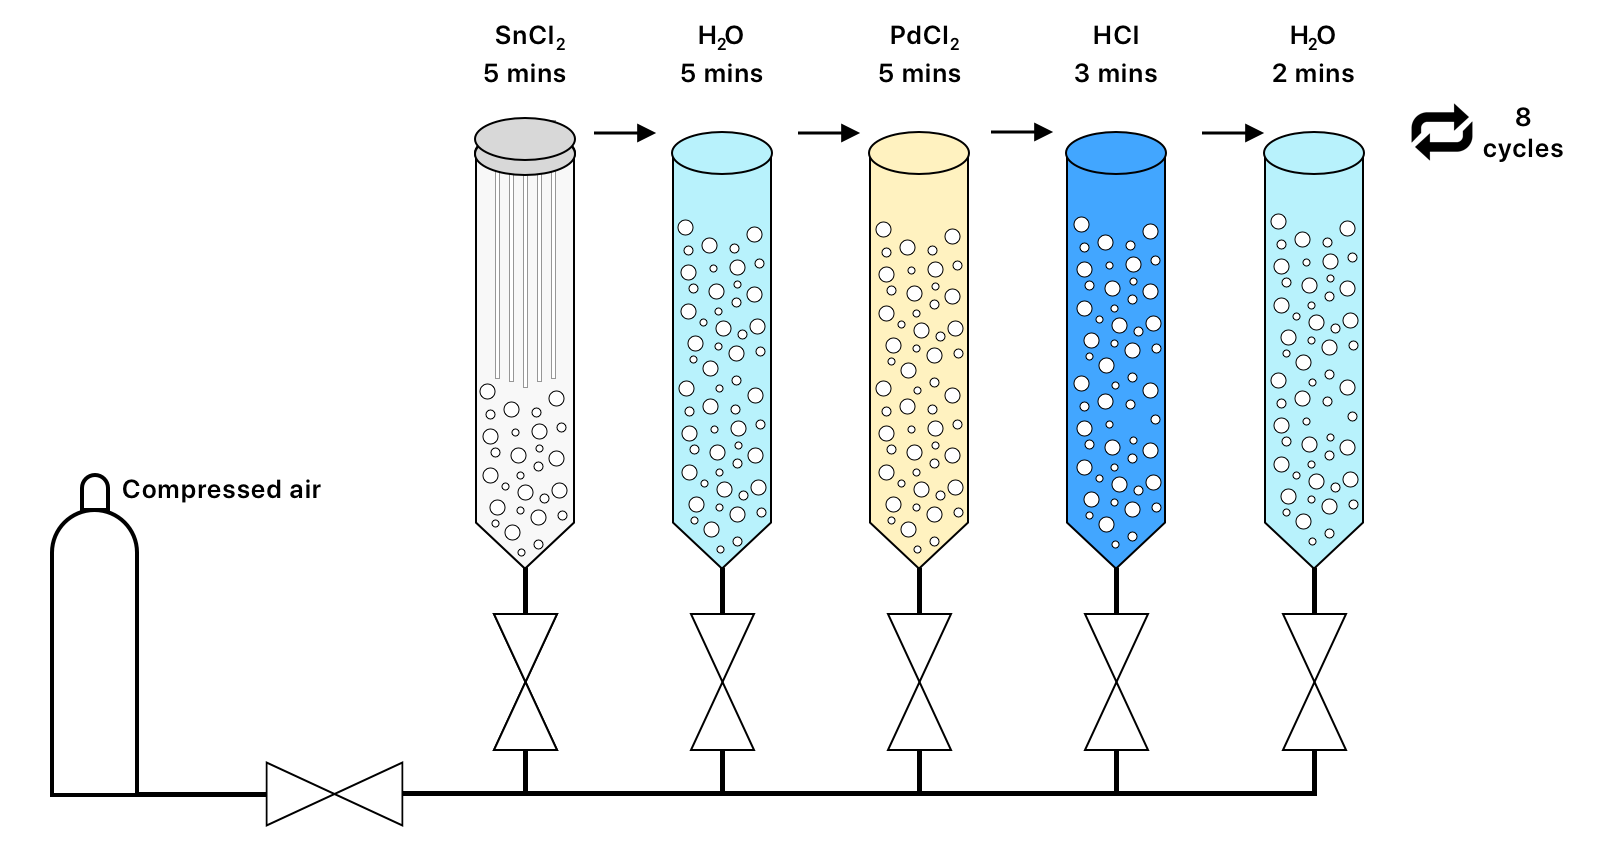
\includegraphics[width=\linewidth]{figures/pretreatment.png}
    \caption{Schematic representation of the sequential baths for sensitisation/activation process.}
    \label{sintering}
  \end{figure}

The substrates were then immersed in a Pd electroless plating (ELP) solution, at 60\textdegree C, in order to deposit metallic Pd layers onto the activated surface. The Pd ELP solution was prepared according to the composition presented in Table \ref{ELP} taken from \cite{GouveiaGil2015} for Pd, \cite{Braun2014} for Ag, \cite{Pomerantz2009}  and left to stabilize for 1 h in an ultrasonic bath prior to use. The volume of Pd ELP solution was fixed at 4 mL per cm\textsubscript{2} of 
substrate surface area. The electroless plating procedure was performed twice, with a total plating time of 60 mins.

After the palladium coating the membranes were then subjected to one, or multiple, other plating steps of silver, gold, or copper. The plating time for silver was 30 minutes for one cycle and the volume of plating solution to substrate was the same as the palladium steps.

It should be noted that the deposition of gold is through immersion plating rather than electroless plating. \cite{adawiyah_azlina_fadil_aisha_hanim_2016} Immersion plating is the process of applying adhering layers of nobler metals to another metal's surface by dipping the material in a heated nobler metal solution ion to produce a replacement reaction. This causes the deposition of a metallic coating on a base metal from solutions that contain coating metal. One metal is typically displaced by metal ions that have lower levels of oxidation potential, relative to the metal ion being displaced. The plating time for gold was 3 hours and the volume of plating solution to substrate was 4mL/cm\textsuperscript{3}. 

The resulting composite membranes consisting of multiple metal layers stacked were then heat treated at 500\textdegree C under an environment containing 25\% H\textsubscript{2} in Ar balance for 24 hours in order to alloy the layers into a homogenous membrane and reduce any oxides that were present on the surface.


\begin{figure}
    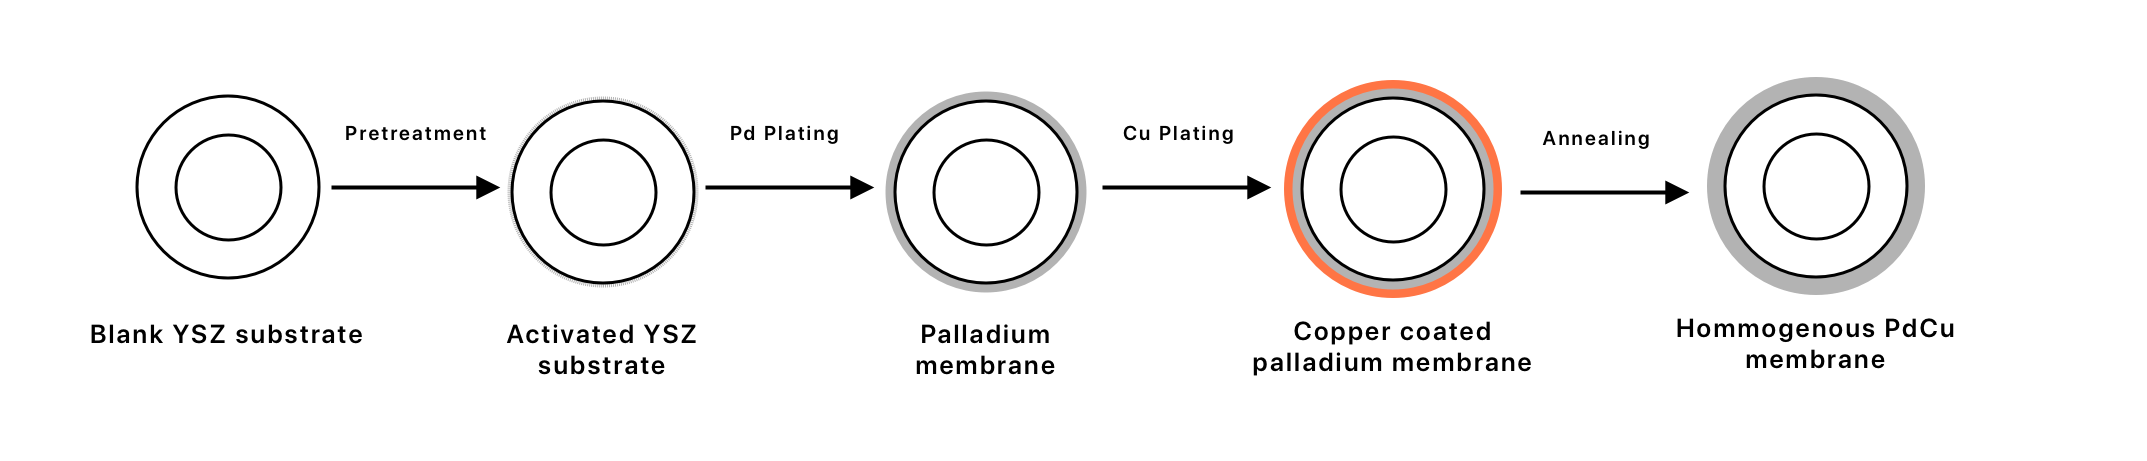
\includegraphics[width=\linewidth]{figures/ELpprocedure.png}
    \caption{Example of ELP procedure when manufacturing a PdCu membrane on YSZ substrate}
    \label{ELP Procedure}
  \end{figure}

\subsubsection{Magnetron Sputtering}\label{msproc}
Membranes were deposited using a closed field unbalanced magnetron sputter ion plating system produced by Teer Coatings Ltd. The thin film membranes were deposited onto the YSZ 3\% hollow fibres by mounting them vertically inside the sputtering system. The system was then evacuated to 1x10\textsuperscript{-6} mBar and subjected to an ion cleaning process with Ar plasma prior to sputtering. Pd, Cu, and Zr targets (99.9\% purity) were used to sputter the chosen alloy composition onto the membranes at the target currents shown in. A bias voltage of 50 V was applied to the magnetron during deposition runs. Samples were deposited using pulsed DC, with a constant target to substrate distance and a sample rotation speed of 16 rpm. An Ar flux of 25 (SCC/m) was used during deposition. PdCu membranes in both BCC and FCC phase were manufactured through magnetron sputtering along with PdCuZr ternary alloys. 

\begin{table}[]
    \centering
    \caption{Conditions used during magnetron sputtering of palladium membranes on YSZ tubular substrate}
    \label{sputtering}
    \begin{tabular}{@{}cccc@{}}
    \toprule
    \multirow{2}{*}{Alloy} & \multicolumn{3}{c}{Target current (A)} \\
                           & Pd          & Cu          & Zr         \\ \midrule
    PdCuZr                 & 1.25        & 0.65        & 0.4        \\
    PdCu (fcc)             & 1.25        & 0.8         & -          \\
    PdCu (bcc)             & 1.2         & 1.0         & -          \\ \bottomrule
    \end{tabular}
    \end{table}

\subsection{Materials testing}\label{MatTest}
The thickness of the plated layers was characterised by first using a Focused Ion Beam (FIB) to mill through a section of the hollow fibre to provide a flat, cross sectional surface for analysis. The thickness of the metal later was then measured using high resolution Scanning Electron Microscopy (SEM) and composition analysed using Energy Dispersive x-ray Spectrometry (EDS) on the same sample. 

The surface composition of the membrane was further characterised using X-ray Photoelectron Spectroscopy to provide a more accurate compositional analysis for the top 10 nm of the membrane, the depth which is most relevant for catalytic dissociation of hydrogen and adsorption of impurities.

Prior to the H\textsubscript{2} permeation tests, the integrity of the hollow fibre membranes was evaluated by testing the gas-tightness of the membrane under N\textsubscript{2} atmosphere, up to 10 bar and room temperature and using a gas-tightness apparatus developed in house. \cite{GouveiaGil2015}

\section{Membrane Characterization}

\subsection{Membrane testing rig}
After the membranes were ensured to be gas tight, hydrogen permeation measurements were performed using the experimental apparatus shown in Figure 1. The palladium alloy composite hollow fibre membranes were sealed on to a stainless steel ¼” NPT fitting. The membrane was then placed in a Sulfinert®-treated sample vessel (Thames Restek, UK) with nominal volume of 300 cm\textsuperscript{3}. The vessel was then heated using heavy insulated heating tape (OMEGA STH051-020). The heating was controlled using the temperature of the membrane using a PID temperature controller (OMRON). The feed was supplied from a cylinder either containing BIP+ hydrogen (Air Products) for pure hydrogen permeability tests or one of two gravimetrically prepared gas mixtures for impurity testing shown in tables \ref{nonsulf} and \ref{sulf}. Prior to introducing gas to the membrane the system was evacuated down to 1 x 10\textsuperscript{-6} mbar. The pressure on the retentate side of the membrane is controlled using a tamper proof pressure reducer. The set-up is shown in figure \ref{testrig}. After tests the system was vented and purged 7 times with N\textsubscript{2} to ensure an explosive atmosphere could not build up within the equipment.

The flux and permeability of the membrane were automatically calculated using software developed in house. Each membrane sample was made using the same batch of substrate and cut to the same length prior to testing. The permeability (P)  of a dense metal membrane is given by Eqn \ref{eq:1} \cite{NathanW.Ockwig2007} and is a function of the hydrogen flux through the membrane (J), the concentration and pressure gradient across the membrane ($P^{0.5}_{ret}-P^{0.5}_{perm}$), and the thickness of the metallic membrane (l). 

\begin{equation} \label{eq:1}
    P = \frac{J l}{P^{0.5}_{ret}-P^{0.5}_{perm}}
\end{equation}

\begin{landscape}
\begin{figure}[h]
  \centering
  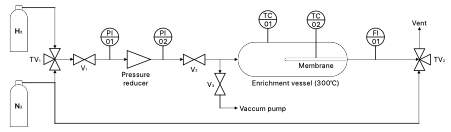
\includegraphics[decodearray={0.2 0.5}, width=0.9\linewidth, height=\textheight,  keepaspectratio]{/Users/marc/Thesis/Experimental/perm_rig.png}
  \caption{Experimental set up used during hydrogen permeation and enrichment experiments, TC: Temperature controller, PI: Pressure indicator, V: Valve, TV: Three-way valve,  FI: Flow indicator.}
  \label{testrig}
\end{figure}

\end{landscape}

\section{Hydrogen impurity enrichment}\label{enrichproc}
A hydrogen impurity enrichment device was designed and tested, more details on this will be discussed in chapter 6. This section will describe the methodology and testing procedure for the hydrogen impurity enrichment device. 

Hydrogen impurity enrichment tests were performed on synthetic samples created using the procedure described in section \ref{gasprep} and using a sample taken from a hydrogen refuelling station. Regardless of source all samples were tested using a PDHID in order to calculate it's oxygen level for safety reasons. Since only hydrogen can leave the HIED in normal testing conditions, if not checked the concentration of oxygen could rise above a safe level and create an explosive mixture. For the purpose of these tests the enrichment factor was capped at a value that would ensure the oxygen level in the mixture would not surpass 1\%. 

The enrichment factor was calculated using both non-ideal gas law (equation \ref{lit-eq:1}), and tracer enrichment (equation \ref{lit-eq:2}) methods. This was to ensure any leaks in the device could be detected using non-ideal gas law method, while having a low uncertainty on the final value from the tracer enrichment method. Gas composition testing was performed using the same GC procedures discuessed in section \ref{gasprep}
\subsection{Krypton spiking}
In order to perform enrichment using the tracer enrichment method a certain quantity of inert gas, not normally present within a hydrogen sample, must be included in the gas. Krypton was used in this study. For synthetic samples this can be added using loop addition along with other impurities using the procedure in section \ref{gasprep}. When taking a sample directly from a hydrogen refuelling station, as would have to be done in real sampling, this approach is not effective as the tracer gas cannot be added to an already pressurised container. The krypton must first be added to the evacuated sampling vessel through loop addition.

Since sampling from a hydrogen refuelling station is dependent on a number of variables, it is difficult to determine the final pressure of the sample. Therefore, a fixed quantity of krypton gas was added to the cylingers. For the purpose of this thesis, since 10L cylinders were used for the purpose of hydrogen sampling, 0.3g of Kr was added through loop addition as this is enough to ensure at a max fill pressure of 100 bar there would be atleast 70 \textmu mol/mol, which is well within the range of the GC-PDHID detector, and avaliable gas standards for validation. 

\subsection{Performing enrichment}
The protocol for performing hydrogen impurity enrichment is similar to hydrogen permeation tests. After evacuation the gas is introduced to a vessel containing the chosen palladium membrane composition at a set enrichment pressure and the vessel heated to 300\textdegree C to begin enrichment. The pressure of the enrichment vessel and sample cylinder were both monitored and their values used to calculate the enrichment factor in real time using equations \ref{lit-eq:1} and \ref{lit-eq:2}. 

Once the desired enrichment factor was achieved the heater was switched off and the enrichment vessel isolated. The enrichment vessel was then brought to the desired GC detector and tested in the GC-PDHID as described in section \ref{gasprep} in order to determine the krypton composition against the original sample, and gas standards. This krypton concentration is used to calculate the tracer enrichment factor. The concentration of other impurities in the enriched sample can then be quantified by testing the enriched sample against a gas standard containing the target impurity, and it's original composition calculated using this value in conjunction with the tracer enrichment factor. 

The uncertainty for both non-ideal gas law, and tracer enrichment factor, and their effect on the final composition calculated using these methods. For non-ideal gas law method the sources for uncertainty arise from errors associated with the sensors monitoring process variables, namely temperature and pressures, in addition to the uncertainty with the method used to correct for non-ideal gas behaviour, and the uncertainty associated with the gas analysis equipment used to determine the composition of both the enriched, and unenriched samples. For tracer enrichment the only source of uncertainty is from the gas analysis equipment used to determine the composition of the enriched and unenriched gas. Values for these errors can be found in Appendix 3

\section{Density functional theory} \label{DFTparams}
All DFT calculations were performed using the Quantum Espresso (QE) \cite{QE-2009, QE-2017, doi:10.1063/5.0005082} ab initio simulation package using the generalized gradient approximation with the PW91 functional to describe electron-correlation effects. Ion-electron interactions were described using ultra-soft pseudopotentials. A plane-wave expansion with a cut-off energy of 233.73 eV was used in all calculations. Geometry relaxations were performed with a conjugate gradient method until the forces on all unconstrained atoms were less than 0.03 eV/A. A Monkhorst Pack mesh with 5x5x5 k-points was used for all calculations as this was determined to be adequate for achieveing convergence from literature in table \ref{lit-DFTREV} and backed up by initial testing on a Pd system as shown in figure \ref{kpoints}.

\begin{figure}
  \centering
  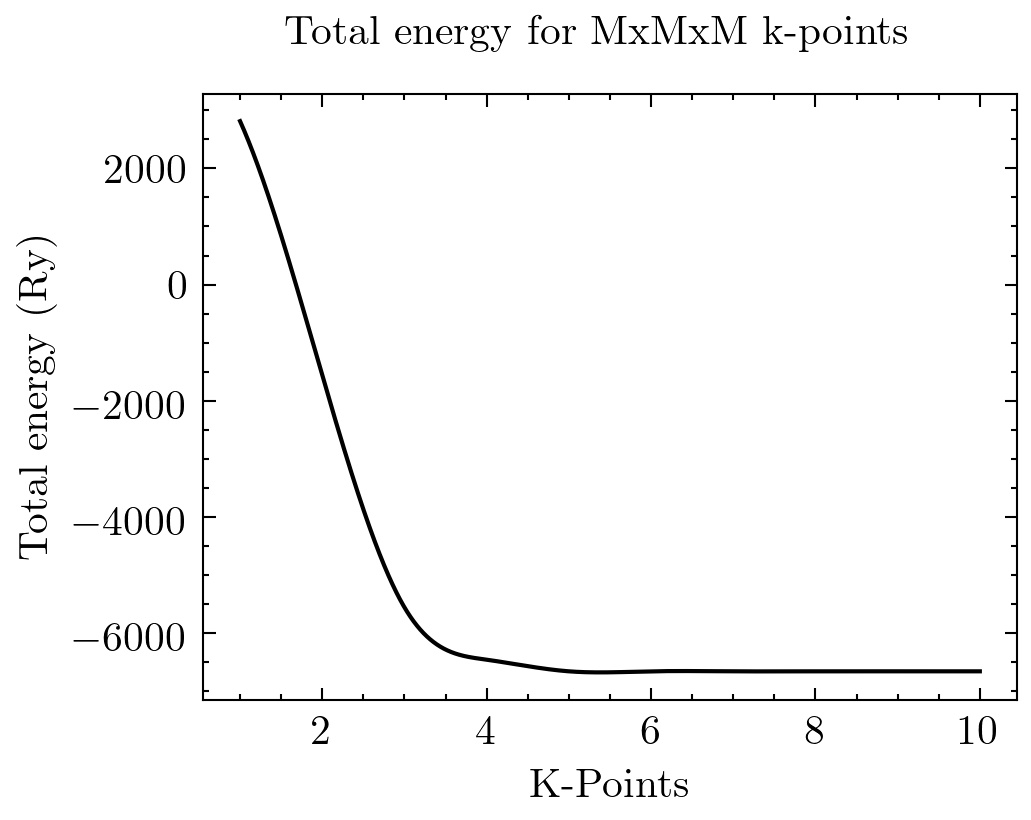
\includegraphics[width=\linewidth, height=0.45\textheight,keepaspectratio]{/Users/marc/Thesis/Experimental/kpoints.jpg}
  \caption{Total energy as a function of $M\times M\times M$ k-points across a Pd(111) fcc slab}
  \label{kpoints}
\end{figure}

Python with scikit learn, pandas, numpy, and matplotlib packages were used for scripting, data collection and analysis. Sample files can be found in Appendix 3. 

\subsection{ISO 14687 Impurities and Hydrogen} \label{gassim}
ISO 14687 impurities were simulated using the above parameters and their structure relaxed until convergence was achieved. The resulting structure was then cross checked using bond lengths from literature to ensure the resulting molecule was an accurate representation. 

\subsection{Palladium and Palladium alloy slab models}\label{slabsim}
The structure of bulk palladium was first created using a lattice parameter of 3.859\si{\angstrom} as reported by D. Wheeler \cite{PhysRev.25.753}. Initially the pure palladium slab model used to represent the periodic supercell was created using this palladium primative unit cell cleaved using the miller indices $(h,k,l) = (111)$ which is adequate in describing the surface of a palladium membrane. A $2\times 2$ slab was created in order to ensure minimal in-plane interactions between neighbouring molecules adsorbed onto the surface in the periodic simulations. The slab was extended to 5 atom thickness which is adequate to describe the surface of Pd(111) and a 20\si{\angstrom} vaccum layer was placed on top. The resulting supercell consisted of 20 atoms. 

When creating palladium alloy systems it was assumed that alloys adopt a substitutional, random fcc structure. Metal atoms were randomly distributed among the fcc lattice in the supercell. All atoms were allowed to relax during the calculation, with the volume of the super cell fixed. 

Quantum ATK Virtual NanoLab Builder \cite{synopsys} was used to generate these structures and export to QE input files. Each metal composition was simulated with three random distributions of substituted metal. For each alloy, geometry optimization was performed to get the lattice constant and total energy of each alloy prior to adsorption of gaseous molecules.

\subsubsection{Adsorption energy}
In order to find the adsorption energy of each ISO 14687 impurity on the membrane surfaces the molecules simulated in section \ref{gassim} were inserted into the vacuum region of the slab models generated in section \ref{slabsim}. (111) fcc surfaces have 4 available sites for adsorption shown in figure \ref{lit-fccsites} A separate system was created for adsorption of each impurity onto each of these sites. Initially the adsorbed molecule was simulated using a ridgid constraint to prevent any changes to the impurities molecular structure, and a low cutoff energy in order to get a quick starting point for the basis of the full simulation. Final goemetry relaxation was then performed from this using the parameters described in section \ref{DFTparams}

The adsorption energy, $E_{i_{ads}}$, for the adsorption of a gaseous impurity on the surface is then calculated using equation \ref{lit-adseqn} where $i$ is the target ISO 14687 impurity or hydrogen molecule.

\renewcommand{\bibname}{References}
\bibliographystyle{unsrtnat}
\bibliography{library.bib}